\chapter{实证研究方法}\label{research_method}
    \section{期权的定价模型}
    本文首先采用Black-Scholes模型对比特币进行定价。Black-Scholes模型对交易资产及其市场有如下假设:
    \begin{itemize}
        \item 存在已知且恒定的无风险收益率r。
        \item 资产价格为带漂移随机游走过程, 即$dS={\mu}Sdt+{\sigma}SdW$,其中价格波动率$\sigma$为已知的常数。可以推导出在这一假设下资产的收益率服从对数正态分布。
        \item 期权为欧式期权,即只有到期时期权的购买者才能够行权。
        \item 买卖期权和标的资产时不会产生交易费用和其他损失。
        \item 能够以无风险利率自由借入借出任意数量的资产。
        \item 对卖空操作无限制。
        \item 不存在无风险套利机会。
        \item 资产不支付红利。
    \end{itemize}
    在以上假设下,可以得到如下的期权定价公式:
    \begin{equation}\label{bs-call}
            C=S*N(d_1)-X*e^{-rT}*N(d_2) 
    \end{equation}
    \begin{equation}\label{bs-put}
        P=X*e^{-rT}*N(-d_2)-S*N(-d_1)
    \end{equation}
    其中
    \begin{equation*}
        \begin{split}
        d_1=\frac{ln(S/X)+(r+\sigma^2/2)T}{\sigma{\sqrt{T}}} \\
        d_2=\frac{ln(S/X)+(r-\sigma^2/2)T}{\sigma{\sqrt{T}}}
        \end{split}
    \end{equation*}
    其中,C为看涨期权价格,P为看跌期权价格,S为标的资产价格,X为行权价格,r为无风险利率,T为距离到期日时间,$\sigma$为资产收益率的波动率。
    
        比起股票或其他传统金融资产,比特币市场一定程度上更符合Black-Scholes模型的假设,也更利于进行推导模型时构建的delta-对冲过程:
        \begin{itemize}
            \item 比特币为连续交易,无假日和休市时间,可以在任意时间买卖。
            \item 比特币可以分割成(足够小的)任意单位买卖,而非必须整数。
        \end{itemize}

    \section{波动率的估计}
    现实中,市场上的真实波动率并非恒定且已知的,因而无法直接采用\ref{bs-call}\ref{bs-put}的公式对期权进行定价。主要可以采用如下几种方式对价格波动率进行估计。
    \subsection{波动率滚动估计}
    投资者在市场上直接观察到的是近期一段时间比特币价格的波动。可以利用滚动窗口得到近期收益率的标准差估计,并将其作为期权到期日期前的期望波动率:
    \begin{equation}\label{volatility-rolling}
        \hat{\sigma}=\sum_{i=1}^{i=N}\frac{(r_{t-i}-\bar{r})^2}{N-1}
    \end{equation}
    其中$\bar{r}$为这一时期的平均收益率。本文中采用以一年(365天)为滚动窗口估计。用此方法得到的波动率估计相对稳定,同时也能反映出短期的波动趋势,数据期内估计波动率的变化如图\ref{fig:volatility}:
    \begin{figure}[H]
        \begin{small}
            \begin{center}
                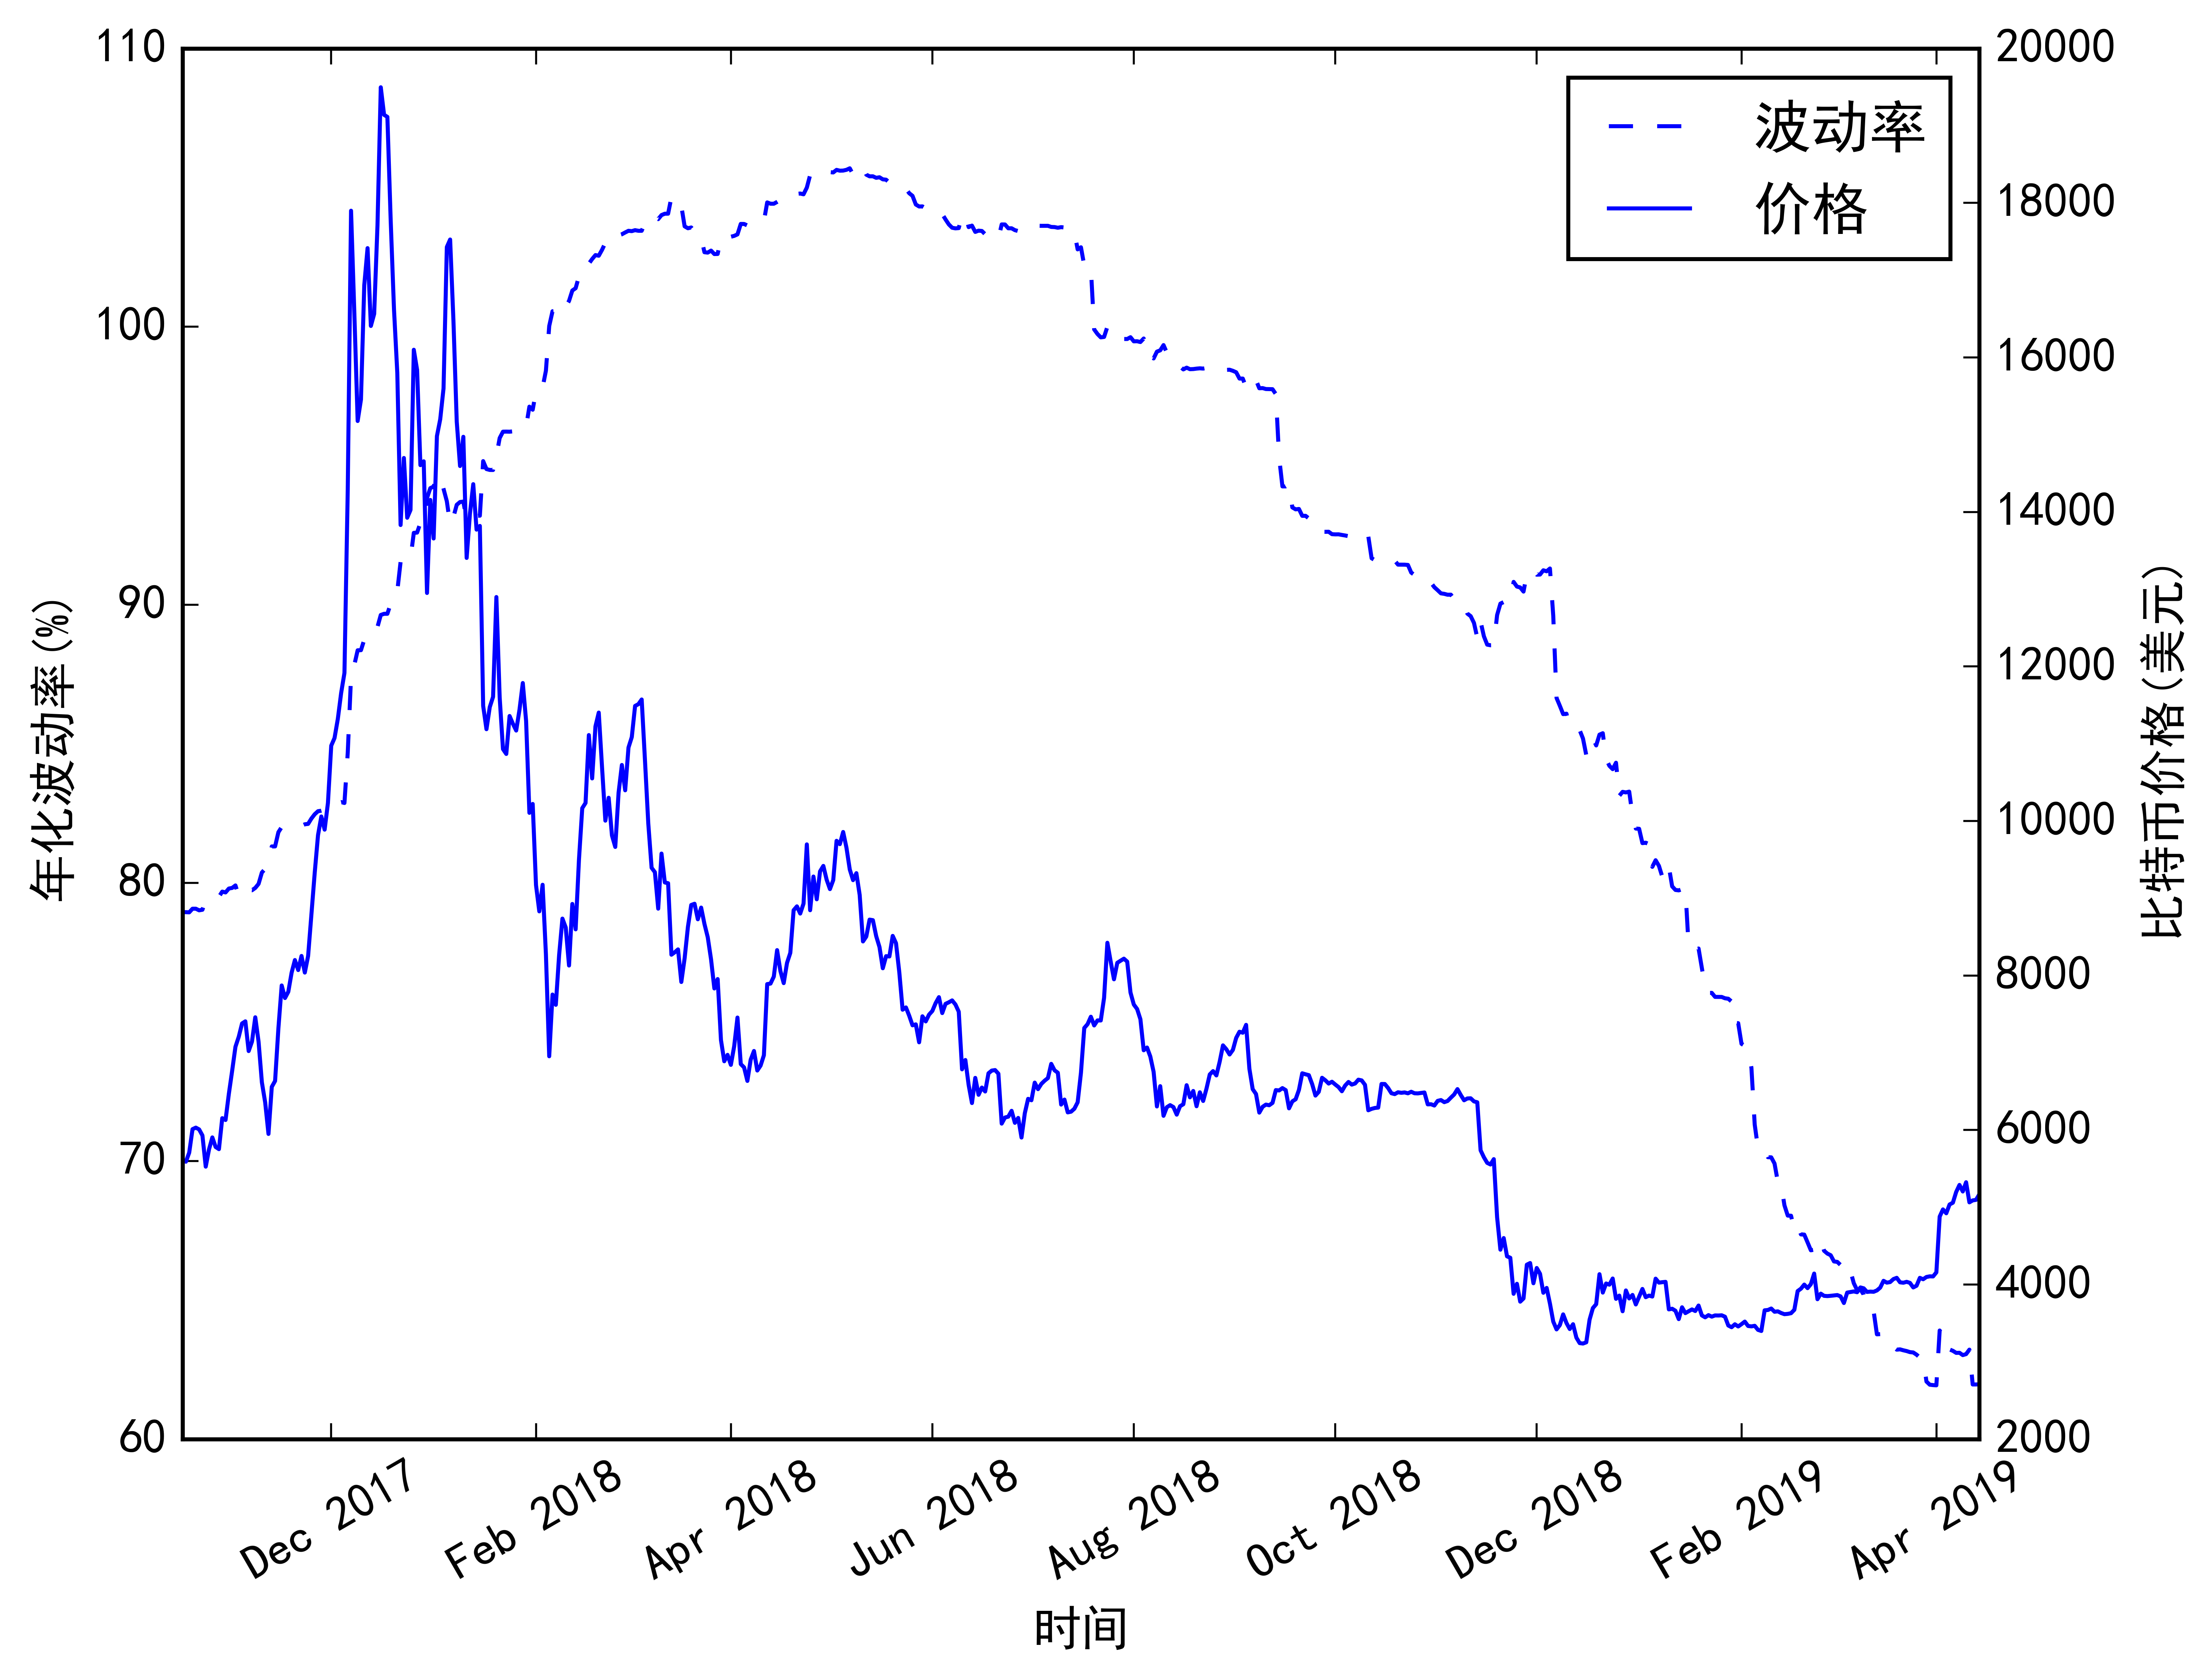
\includegraphics[width=0.95\textwidth]{figures/volatility.png}
            \end{center}
            \caption{数据期内比特币收益率滚动估计波动率}
            \label{fig:volatility}
        \end{small}
    \end{figure}
    这一估计充分捕捉到了2018年中的高波动率与18年末的低波动率,是目前比较好的对比特币收益波动的估计方式。
    \subsection{加权隐含波动率估计}
    从式\ref{bs-call}和\ref{bs-put}可以得出,期权的价格随波动率上升而上升。可以通过现在市场上的均衡期权价格得到一个$\sigma$的解,即为隐含波动率,这一预测方法利用了期权交易中的隐含信息。
    根据参考文献\cite{CHIRAS1978213},每日有多支期权且他们隐含波动率不同时,可以用以下公式获得当日的加权隐含波动率(WISD):
    \begin{equation}
        WISD=\frac{\sum_{j=1}^{N}{ISD_j\frac{\partial{W_j}}{\partial{v_j}}\frac{v_j}{W_j}}}{\sum_{j=1}^{N}{\frac{\partial{W_j}}{\partial{v_j}}\frac{v_j}{W_j}}}
    \end{equation}
    其中 , $WISD$为加权隐含波动率,$ISD_j$为第$j$个期权的隐含波动率,$N$为同一标的资产的期权个数,$\frac{\partial{W_j}}{\partial{v_j}}\frac{v_j}{W_j}$ 为期权价格相对于波动率的弹性。
    \par{考虑到目前期权交易占整个比特币市场的交易比重并不大,故使用这一方式可能并不能有效反映期权定价中的波动率信息。}
    \section{对定价偏差的解释}\label{reg vars}
    波动率微笑现象反映出了期权的隐含波动率和其价值程度(即资产价格与行权价之比)存在规律性的关系,同理我们可以探究很多变量对于期权真实价格与模型价格之间偏差的系统性影响。通过构建回归模型并对变量的系数进行分析,我们可以识别不同因素对真实价格偏离部分的影响的方向,并对其做出解释。这些变量主要分为两个方面:比特币市场因素和期权因素。
    \subsection{比特币市场有关变量}
    \begin{itemize}
        \item log\_ret 比特币市场对数收益率
        \item volatility 比特币历史波动率
        \item skewness 比特币收益率历史偏度
        \item kurtosis 比特币收益率历史峰度
        \item amihud Amihud非流动性指标
        \item btc\_volume 比特币市场总交易量
        \item maxmin\_ratio 当日比特币交易所中价格最高者和最低者之比
    \end{itemize}
    
    这些指标衡量了比特币市场的市场环境。如波动率、偏度、峰度反映了投资者所处的风险情况,同时也属于识别出的模型设定问题,偏度和峰度的存在影响了而非流动性指标和MR体现了市场的流动性情况,这些都可能造成真实价格同模型价格之间的偏差。
    \subsection{期权自身有关变量}
    \begin{itemize}
        \item delta 期权根据Black-Scholes模型计算出的delta
        \item time 期权距离到期日的时间
        \item vol\_pre 期权的波动率溢价(Volatility Premimum),利用该期权当时的隐含波动率与当天至到期日之间的实现波动率之差计量。
        \item volume 期权当天交易量                                     
        \item spread 期权当天公开的买卖价差
        \item open\_interest 期权当天公开的持仓量
        \item contract\_is\_call 哑变量,是否为认购期权,1为认购期权,0为认沽期权。 
    \end{itemize}
    这些指标能够衡量期权自身性质对真实价格的影响,主要是不同性质的期权可能导致投资者对其供给和需求的不平衡会造成期权价格的偏离。
    \section{套利策略}\label{strategy}
    B-S模型是基于用股票和无风险债券复制期权而没有套利空间的原理推导出来的。由此可以利用实际价格与模型价格偏离的部分,构建套利策略,这一策略将反映出B-S模型中包含的信息价值。根据已有的B-S模型计算delta值后,策略详情如下:
    \begin{itemize}
        \item 对于一只期权,有交易记录的一天即用实际价格和B-S模型价格比较,实际价格高于模型价格的,卖出期权,同时买入delta份比特币进行对冲;实际价格低于模型价格的,买入期权,同时卖出delta份比特币进行对冲。记录现金流。
        \item 在第二天\footnote{当期权的交易数据不是连续时,选择该期权下一条有交易的日期,一般间隔不会太大。}清空已有的持仓(包括期权和股票),同时重新构建新的资产组合。如果第二天为该期权的行权日,则视比特币价格与行权价之间的关系选择是否行权。完成后记录现金流。
        \item 将一只期权各个时点上(构建期权和清空仓位的日期)的现金流按照模型采用的无风险收益率(年化5$\%$)折现至起始日期,并计算入现金流-出现金流。
    \end{itemize}
    除了行权日期之外,这一策略每次建仓至平仓的收益可以表示为:
    \begin{equation}
        \Delta{P}-\delta{\Delta{S}}-(P-\delta{S})r\Delta{t}
    \end{equation}
    其中,P为期权建仓时价格,$\Delta{P}$为前后期权价格变化,$\Delta{S}$为前后比特币价格变化,r为无风险利率。
    根据参考文献\cite{Hull-2017},考虑到价格和波动率之间的相关性,可以通过修正由B-S模型简单计算出来的delta的方式来实现优化的对冲比率。推导得到的最优对冲比率$\delta_{MV}$\footnote{此处的最优指的是期望的最小方差}为:
    \begin{equation}\label{MVmodel}
        \delta_{MV}=\delta_{BS}+\frac{\gamma_{BS}}{S\sqrt{T}}(a+b\delta_{BS}+c\delta^2_{BS})
    \end{equation}
    其中$\delta_{BS}$为Black-Scholes模型计算出的delta,$\gamma_{BS}$为Black-Scholes模型计算出的gamma。
    实际应用中,可以滚动估计包含delta和delta二次项的线性模型:
    \begin{equation}
        \Delta{f}-\delta_{BS}\Delta{S}=\frac{\gamma_{BS}}{\sqrt{T}}\frac{\Delta{S}}{S}(\hat{a}+\hat{b}\delta_{BS}+\hat{c}\delta^2_{BS})+\epsilon
    \end{equation}
    得到参数之后带入式\ref{MVmodel},可得到此时的对冲误差为:
    \begin{equation}
        \epsilon_{MV}=\Delta{f}-\delta_{BS}\Delta{f}-\frac{\gamma_{BS}}{\sqrt{T}}\frac{\Delta{f}}{S}(\hat{a}+\hat{b}\delta_{BS}+\hat{c}\delta^2_{BS})
    \end{equation}
    根据最小二乘法的定义,如果原有对冲误差和$\delta_{BS}$之间的关系设定正确,则对冲误差$\epsilon_{MV}$的方差已经被最小化。
    